
\section{The Interference of Light}

Name \rule{2.0in}{0.1pt}\hfill{}Section \rule{1.0in}{0.1pt}\hfill{}Date
\rule{1.0in}{0.1pt}

\textbf{Objective}

\begin{itemize}
\item To investigate the interference of light waves as they pass through
a set of slits. 
\end{itemize}
\textbf{Apparatus}

\begin{itemize}
\item Basic optics diode laser
\item Optical bench with rotary motion sensor
\item Phototransistor for measuring light intensity (mounted on rotary motion sensor)
\item ``Multiple Slit Set'' slit accessory
\item {\it Pasco} 550 Interface
\end{itemize}
\textbf{Introduction}

In this laboratory you will investigate the interference of light
produced by a laser beam passing through a set of narrow, adjacent
slits. When light passes the slits each opening acts as an independent
source of waves that can overlap one another to produce a distinctive
pattern of bright and dark spots on a screen. The position of the
bright spots depends on the separation of the adjacent slits and the
wavelength of the incident light. 

The position of these bright spots or interference maxima can be described by

\[
y_{m}=\frac{\lambda L}{d}m\]

where $y_{m}$ is the distance of a bright spot from the central
maximum and $L$ is
the distance from the slits to the screen. The quantity $d$
is the slit separation, \( \lambda  \) is the wavelength of the light,
and $m$ is the order of the bright spot. 

You can measure this interference pattern with the setup shown below. 
(This is a \underline{top} view of the set-up.) 
A phototransistor is seated behind the narrow opening on top of the large,
metal mount sitting on a rail. The phototransistor can translate the intensity 
of the light falling on it into a voltage signal that can be read by the
computer. In addition, the phototransistor can be moved back and
forth on a rotary motion sensor that measures the position of the 
mount. These two signals can be combined to
make a graph of the intensity as a function of position.

\vspace{0.3cm}
%{\centering \resizebox*{0.75\textwidth}{!}{\includegraphics{interferenceOfLight/interferenceOfLight_fig_1.eps}} \par}
%{\centering \resizebox*{0.75\textwidth}{!}{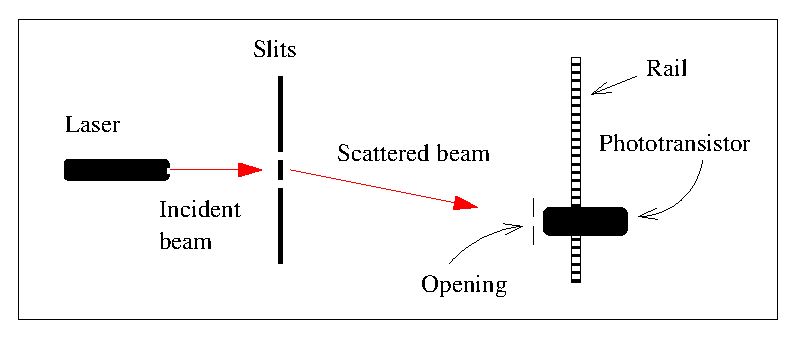
\includegraphics{interference/interference_of_light_fig1c.eps}} \par}
{\centering \resizebox*{0.75\textwidth}{!}{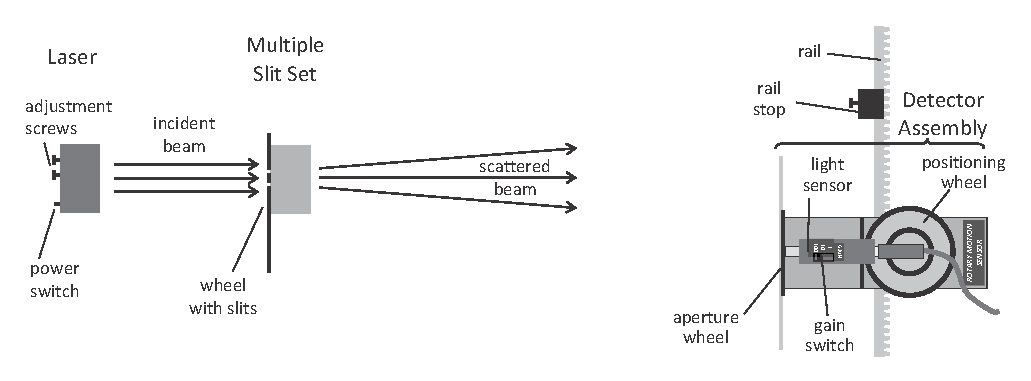
\includegraphics{interference/apparatus.eps}} \par}
\vspace{0.3cm}




In this unit you will pass light from the laser through slits of known
separation and use the interference pattern to determine the wavelength
of the light.

\textbf{Activity 1: An Alternative View}

Isaac Newton believed that light was made up of small, unseen particles
that obeyed (surprisingly enough!) Newton's Laws. This view is known
as the corpuscular theory. We want to consider how this model of light
predicts different behavior from the wave theory.

(a) Consider a laser beam shining on a circular hole. If a beam of
light consisted of small, unseen particles that behaved as tiny billiard
balls what would you see on a screen that is downstream from the circular
hole? A sketch might be useful here.
\vspace{35mm}

(b) Now consider the same laser beam shining on a pair of narrow slits.
What would you see on a screen downstream from the slits if light
were made of corpuscles?
\vspace{35mm}

For the questions above you should have predicted that the laser would
form a single bright spot (for part a) or two parallel lines (for part
b). The experiment you are about to perform provided compelling evidence
that Newton's corpuscular theory was wrong. 
\vspace{7mm}

\textbf{Activity 2: The Interference of Light }

(a) You are now ready to turn on the laser. DO NOT LOOK DIRECTLY INTO
THE BEAM OR POINT THE LASER CARELESSLY ABOUT THE ROOM. Mount the laser on the 
optical bench at the opposite end from the rotary motion sensor. Turn on the
laser and you should see the bright red spot of the beam striking
the rotary motion sensor assembly. On the ``Multiple Slit Set'' accessory, 
select a double slit of width 0.04 mm and separation 0.125 mm marked by the number “2”. 
Rotate the 
wheel so that the double slit is at the center of the opening.
You can rotate the wheel with the slits AND rotate where the slit wheel is mounted
on the plastic frame. Rotate both so that when you click the frame onto the optical bench, the double slit that
you want is at the center of the opening, with the slits oriented vertically and the laser beam centered right on
it. You should now see the “interference pattern” consisting of a series of bright spots a few millimeters apart,
on the white screen in front of the light sensor.

(b) On the light sensor itself, set the small gain switch to “100” (highest sensitivity). Rotate the aperture wheel
in front of the sensor to the position marked “3”. (Wider gaps let in more light; narrower gaps measure light
at a more precisely defined location.) Also check that the sensor is exactly perpendicular to the incident beam;
adjust its mounting if necessary.

(c) Position the double slit about 70 cm from the phototransistor mount. Adjust 
the laser beam direction so that it falls on the double slit you have selected. 
(There are two adjustment screws on the back of the laser.) 
You should see the interference pattern on the phototransistor mount. 
Use the markings on the optical bench to measure the distance from the slits
to the phototransistor case.
Record your value here.
\vspace{10mm}

(d) Position the phototransistor mount so the interference pattern
is at the same height as the opening in the center of the phototransistor mount. 
The phototransistor is mounted behind this hole. 
To make accurate measurements it is important to carefully determine the geometry of your setup. 
Check to see if the slits and the phototransistor mount are perpendicular to the incident
laser beam.  You want to make sure the phototransistor can {}``see'' as many
bright spots as possible. Carefully slide the phototransistor mount 
back and forth to make sure that it stays centered on the interference pattern. 
Then set it at one side of the pattern to begin the experiment.

(e) Open the file {\it Interference.cap} in the {\it Phys132} folder. 
When you are ready, click {\it Record} and slowly move the
detector assembly from one side of the bright spots to the other by rotating the turn wheel on the rotary motion
sensor. Move carefully and take about ten seconds to complete the motion. As you move it, the computer screen
should show a graph of the intensity reading versus the position reading. Click {\it Stop} when you’re done. The
graph, called the interference pattern, should be a symmetric pattern of distinct peaks. Consult your instructor
if your setup isn’t working.
Make a hardcopy of this graph and attach it to this unit.

(f) In the space below, draw a good graph showing your interference pattern. Be sure to label your axes!
\vspace{25mm}

(g) The intensity peaks should appear to be equally spaced. 
Is the spacing between the intensity peaks constant? Is the intensity
of each peak the same? Does it appear that any peaks are missing?
The more peaks you see the more (and hopefully better) data you can collect.
\vspace{12mm}

(h) When you are satisfied with the quality of your spectrum record the 
position of each peak in the left column of the table below, with the central 
peak halfway down the column. You can also create the table in {\it Excel}.
Be sure to print it out when you have filled both columns in and attach it to this
unit.
Use the {\it Coordinates/Delta Tool} 
described in {\it Appendix A} to accurately read off 
the peak positions by clicking on the appropriate button along the top of the 
graph. A set of cross-hairs will appear on the plot. Grab the cross-hairs by 
clicking on them and dragging them to the point you want to measure.
The coordinates will be printed by the cross-hairs.
Turn off the laser when you are finished.

\vspace{0.3cm}
{\centering \begin{tabular}{|c|c|}
\hline 
Position Reading (m)&
Change in Reading (m)\\
\hline
\hline 
&
\\
\hline 
&
\\
\hline 
&
\\
\hline 
&
\\
\hline 
&
\\
\hline 
&
\\
\hline 
&
\\
\hline
&
\\
\hline
&
\\
\hline
&
\\
\hline
&
\\
\hline
&
\\
\hline
&
\\
\hline
\end{tabular}\par}
\vspace{0.3cm}

\textbf{Activity 3: Determining the Wavelength of the Laser }

(a) For the data you recorded in the previous activity, calculate the 
difference between each pair of adjacent readings and record it in the 
right column of the above table (first space will be blank).

(b) Calculate the average and standard deviation of the separation between 
adjacent peaks (right hand column values). Don't forget units.
\vspace{15mm}

(c) The position of each interference maxima is
$$
y_{m}=\frac{\lambda L}{d}m
$$
where $y_{m}$ is the distance of a bright spot from the central
maximum (the distance along the slide in this experiment),
$d$ is the slit separation, and $L$ is
the distance from the slits to the phototransistor. 
The wavelength of the light is \( \lambda  \) ,
and $m$ is the order of the bright spot. 
Generate an expression for
the distance $\Delta y$ between adjacent bright spots.
\vspace{20mm}

(d) Use the expression you generated in part (c) and the average separation
between bright spots you determined in part (b) to calculate the wavelength of 
the laser light and its uncertainty (both in nm). Show how you get the result 
in nanometers. Compare your result with the wavelength range indicated on the 
laser.
\vspace{30mm}

(e) Collect the results for the wavelength from the other teams in class
and calculate the average and standard deviation. Record the results here. 
(Don't forget units.)
Are your results consistent with the class results? Why or why not?
\vspace{15mm}

(f) Recall the earlier discussion of Newton's corpuscular theory of
light. Does your data support Newton's theory or the wave theory?
Why?\vspace{15mm}

